\documentclass{report}
\usepackage{setspace}
\doublespacing
\usepackage[utf8]{inputenc}
\usepackage{graphicx}
\usepackage{amsmath}
\usepackage{indentfirst}
\usepackage[labelfont=bf]{caption}
\usepackage{array, boldline, makecell, booktabs}
\newcommand\btrule[1]{\specialrule{#1}{0pt}{0pt}}
\usepackage{hyperref}
\hypersetup{
    colorlinks=true,
    linkcolor=blue,
    filecolor=magenta,      
    urlcolor=cyan,
}
 
\urlstyle{same}

\title{Polyphase Filter Banks: A Physicist's Attempt}
\author{Matthew Cooper}
\date{May 17th, 2019}
\begin{document}
\maketitle

\tableofcontents{}

\newpage
\chapter{Introduction}

In the modern era, the speed of digital processing components has made it such that the gap between digital and analog is becoming ever smaller, allowing us the advantages that come with conversion of analog signals to digital signals.  These advantages are numerous, but, as with anything, there is an equivalent exchange, and there are tradeoffs in using digital signals which, if not taken into account, can turn a scientific data product into something completely unusable.

In my researching of this subject, it became clear early on that my understanding of the fundamentals that go into digital signal processing (DSP hereafter) were not up to par, which resulted in several hours of researching different aspects of DSP in order to complete the mental picture I needed.  It is my goal in the pages of this report to recreate, as best I can, this journey, making pitstops at different ideas that helped shape my current, albeit incomplete, understanding.  

The first reference I was able to find for polyphase filter bank implementation was a paper from 1973 (Schafer and Rabiner, 1973).  In this paper, however, the term polyphase had not been coined yet.  Its original implementation was to increase the channel edge resolution for speech analyzers in order to create a perfect reconstruction filter.  Not suprising, this came out of Bell Labs.  We'll discuss this paper in greater detail when we come to the theory section.

Although it started as a method of reconstructing speech output, the applications of polyphase filter banks has found use in almost all areas where channelization is required, such as cell phone signal downconversion and up conversion (Harris, 2003), as well as being considered for implementation in the Extended Owens Valley Solar Array.  

In this report, we will review some basics of analog-to-digital conversion, methods which have been created to navigate the restrictions that such conversions place on the type of data which can be sampled, and then proceed with how polyphase filter banks are utilized in the optimization of such a process.  

\chapter{Fundamentals of Digital Signals}
\section{Analog Vs. Digital}

The filtering and manipulation of analog signals has been widely used for decades.  Why, then, is there the push for analog-to-digital conversion?  For systems where the average power of a signal is the only necessity, staying in the analog domain is perfectly acceptable.  The issue arises when a system also needs to accurately measure and record phase information.  In analog systems, the gain to phase balance of a signal cannot be maintained to better than $1\%$ over a range of temperatures (Harris, 2003).  

\begin{figure}[ht]
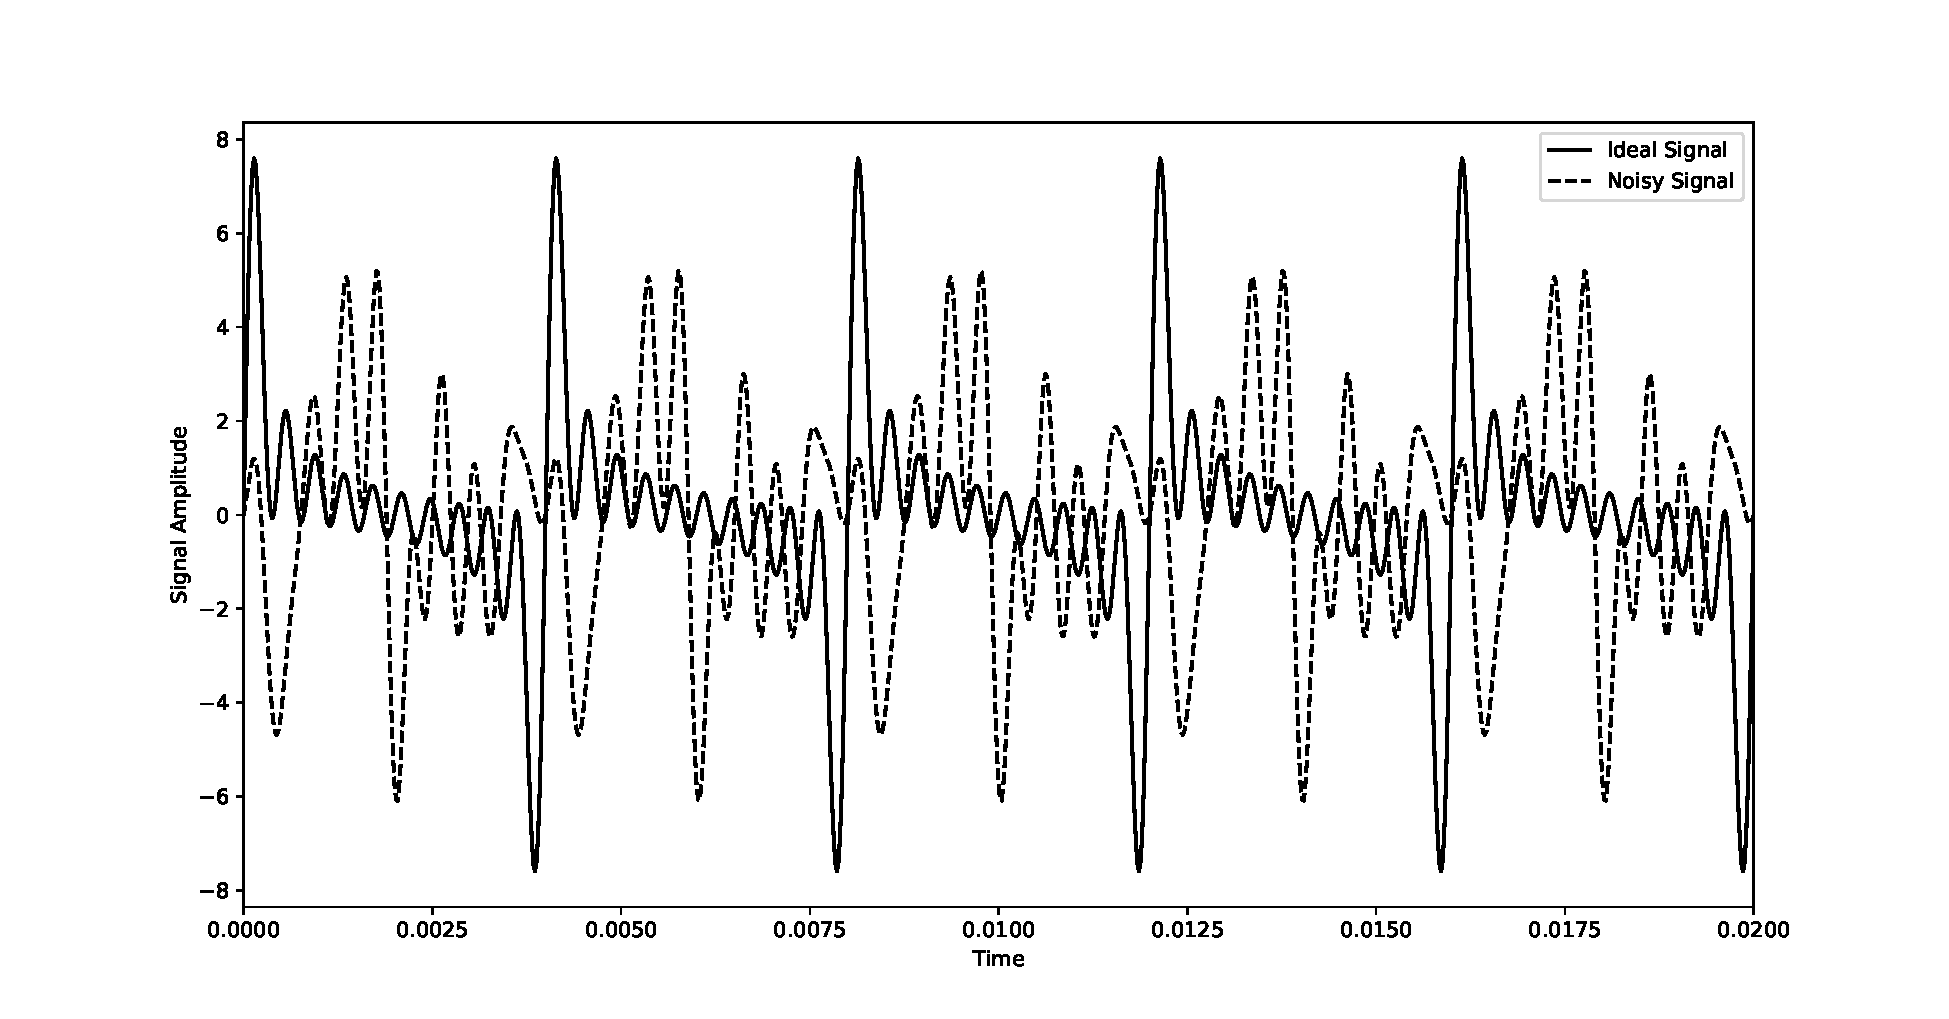
\includegraphics[scale=.45]{Figure_4.pdf}
\caption{Plotted above is an ideal signal which has had uncertainty introduced in its phase and amplitude profile.}
\end{figure}

Figure 1.1 gives an example of the error which can be introduced by such errors.  This is particularily crippling for a multi-antennae radio array, which relies on phase-locking between antennae in order to steer the beam.  Since no two antennae's analog components can match identically, leaving the signal in the analog domain can produce spurious phase shifts, which are functions of many variables which cannot be accounted for simply, if at all.  This is where analog-to-digital conversion is helpful, since the phase information stored in a digital signal is not subject to environmental effects.  

\section{Analog Signal Sampling}

In analog-to-digital conversion, there are two relations which must be considered: the Nyquist Sampling Theorem, and the Frequency Resolution Relation.  These combined determine the sampling rate which must be attained in order to recover a maximum frequency, as well as how much resolution there will be between frequencies.  The Nyquist Theorem (Landau, 1967) states that
\begin{equation}
f_{crit} = \frac{f_{sample}}{2}
\end{equation}

where $f_{crit}$ is the maximum frequency which can have power 'definitively' attributed to it (i.e. has no alias), and $f_{sample}$ is the sampling frequency.  This relation is troubling for radio transmissions.  Consider a 10 GHz signal.  In order to recover this signal, it must be sampled at 20 billion samples per second.  At 64 bit resolution, this equates to around 160 Gigabytes of data.  Currently, FPGA's on the market sit in the MHz processing speed range, although ADC converters currently exist which can handle giga-samples per second.

The second relation, the Frequency Resolution Relation, gives a size requirement for the hardware register which must be fed to the FFT in order to maintain a specific resolution between frequencies.
\begin{equation}
f_{res} = \frac{f_{sample}}{N}
\end{equation}

where $f_{res}$ is the resolvability.  So, for higher sample rates, the register size must also increase to maintain frequency resolvability.  Clearly, a register which is of the order of 160 Gigabytes is something science fiction would hesitate to create, so how is this issue circumvented? The obvious answer is to sample less, but therein lies the problem, since in the process we lose information either by loss of resolution or by ambiguity in frequency aliasing.  The method which was created to address this issue was the concept of downconversion.

\section{Downconversion}

Downconversion (heterodyning) was originally worked on by Nikola Telsa and Reginald Fessenden (Espenschied 1959).  Fessenden patented the heterodyne principle in 1902, and that same year founded the National Electrical Signaling Company (NESCO).  John Vincent Lawless Hogan, who went to work for Fessenden in 1910, showed how the concept had greatly improved the sensitivity of radio receivers (Godara, 1999).  The introduction of this concept revolutionized electromagnetic signaling, and it is no stretch to say that without it, the subject of this paper, as well as many other DSP related ideas, would never have existed.

What is heterodying? Heterodyning is the process by which a signal is mixed with a higher frequency signal in order to mirror the signal to a lower frequency band.  This can be easily shown mathematically.  Consider a monochromatic input signal, $x_{in}$, and a local signal, $x_{lo}$.  Then,
\begin{align}
x_{in}x_{lo}& = sin(f_{in}t)sin(f_{lo}t)\\
             & = \frac{1}{2}[cos((f_{lo}-f_{in})t) - cos((f_{lo}+f_{in})t]
\end{align}

Here, we see that there are two mirrors of the input signal; one which is at higher frequencies, and one which is at lower frequencies, with an example shown in Figure 2.2.  
\begin{figure}[ht]
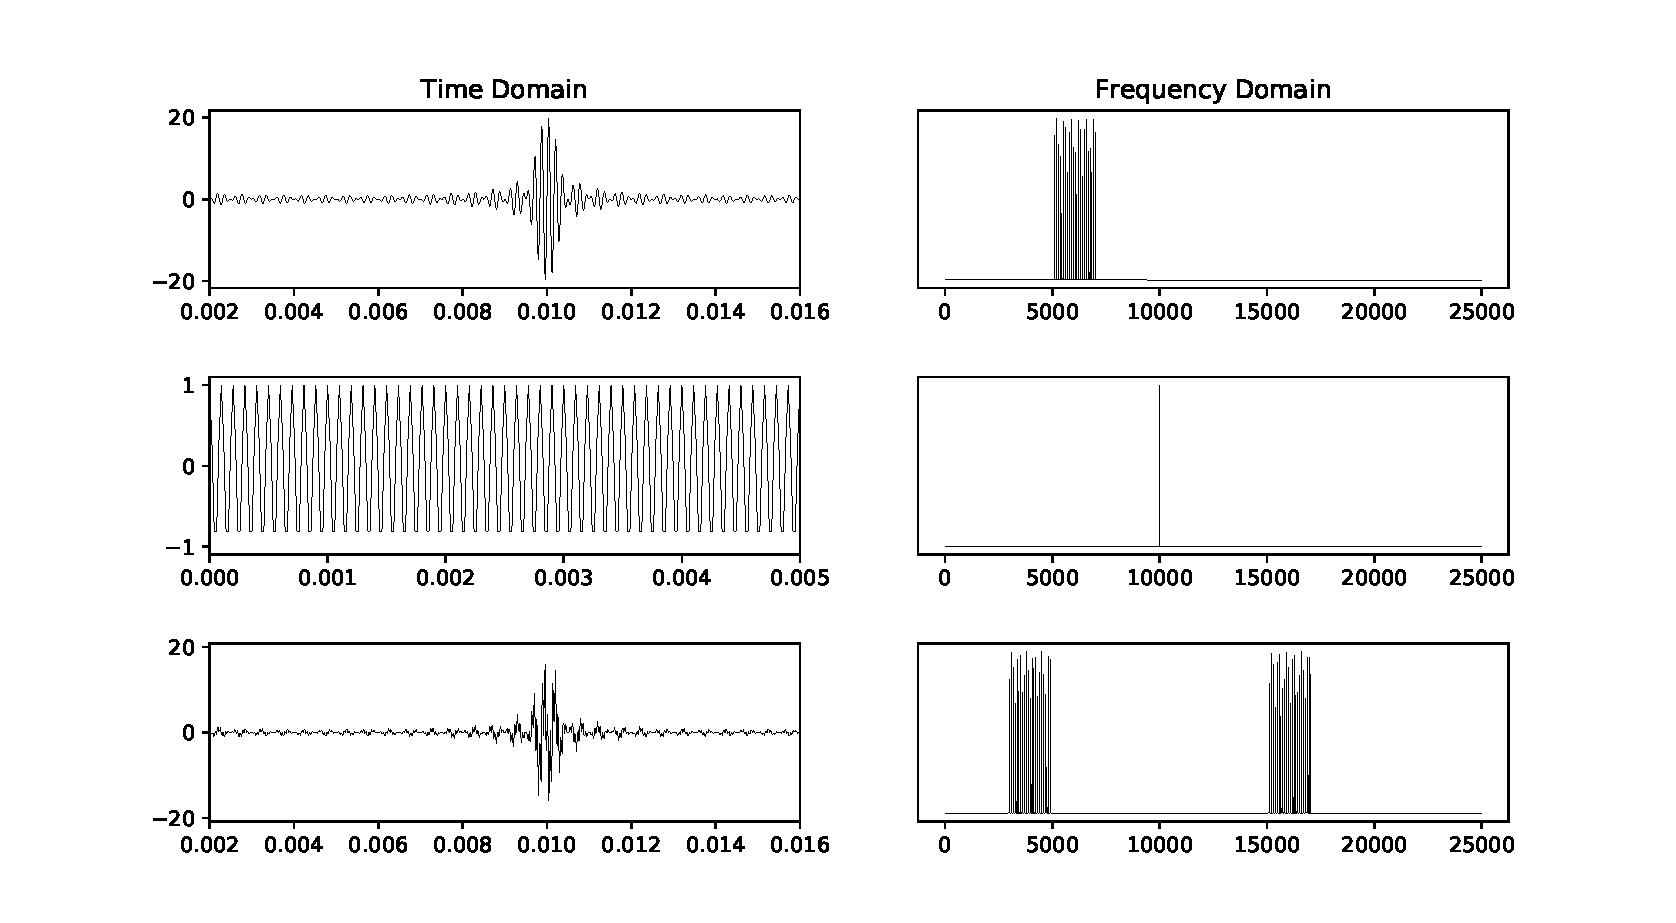
\includegraphics[scale=.45]{Figure_1.pdf}
\caption{(top) Signal $x_{in}$ in the time and frequency domain (middle) Signal $x_{lo}$ in time and frequency domain (bottom) Signal $x_{in}x_{lo}$ in the time and frequency domain}
\end{figure}

The part we are interested in is, of course, the lower frequencies, since we can lower the sampling rate of these frequencies without losing their information.  Therefore, the higher frequency components must be removed.  This is accomplished by convolving the input signal with a transfer function known as a filter function.

\section{Digital Signal Filters}

Digital signal filters are arguably one of the biggest fields within the realm of electrical engineering, and for good reason.  This process allows one to attenuate certain frequency bands, while leaving others (relatively) unaffected. 

\begin{figure}[ht]
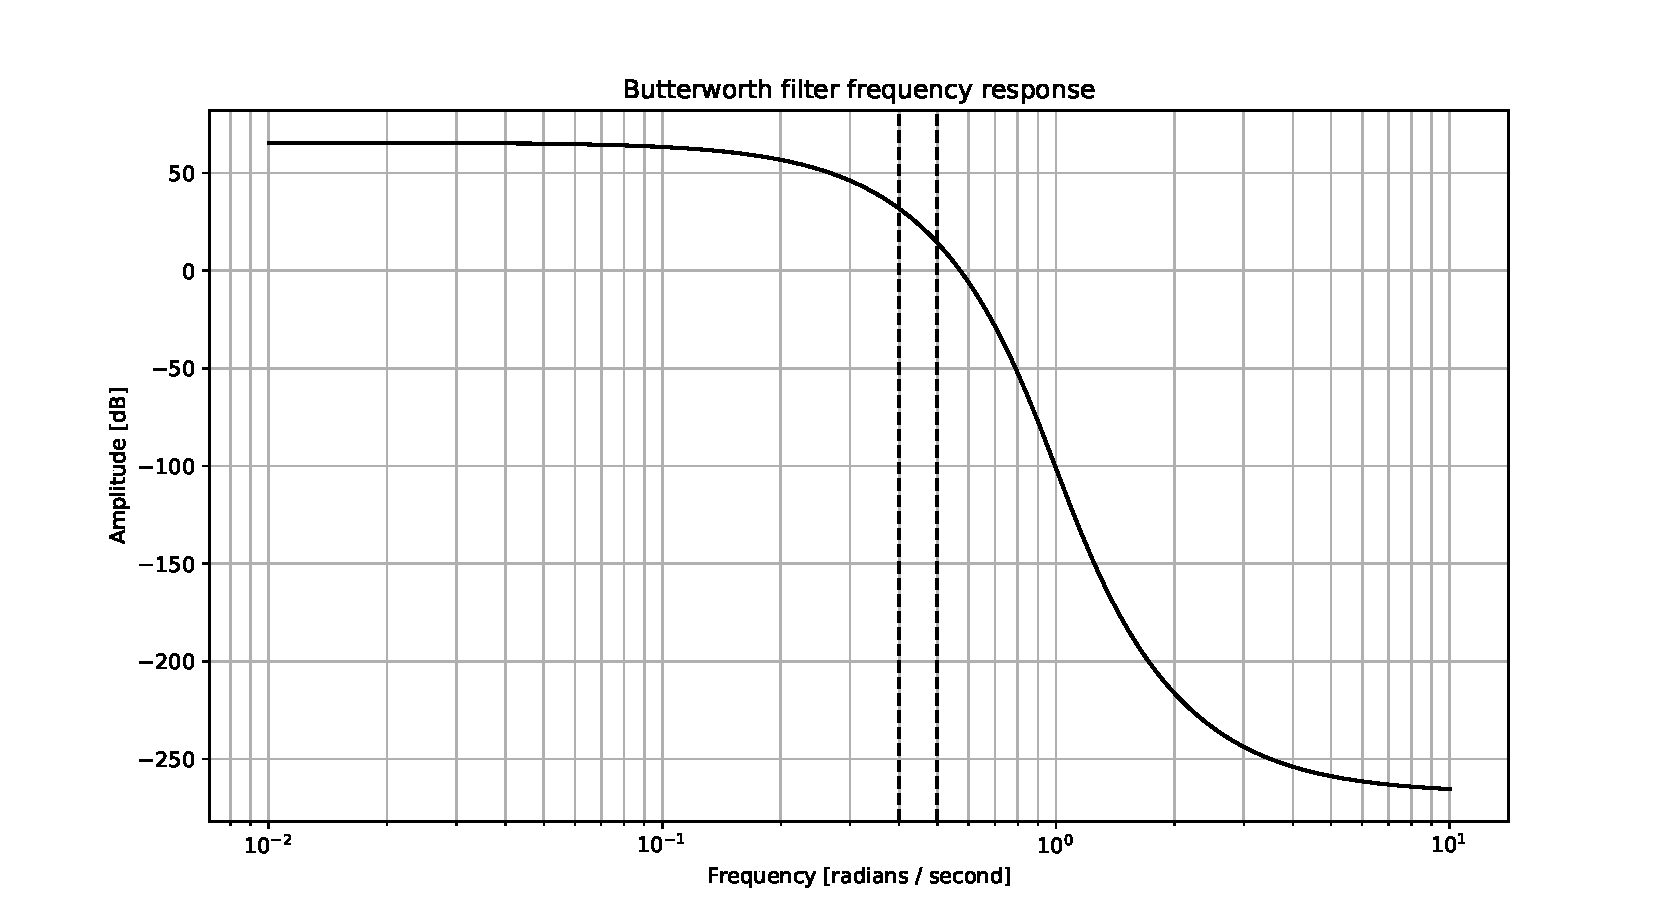
\includegraphics[scale=.45]{Figure_2.pdf}
\caption{Plotted above is the frequency responses for a Butterworth filter of low-pass type.  The y-axis indicated the attenuation (in dB) of the different frequency components.  The first dashed line indicated the end of the pass-band, and the second is the beginning of the stop band.}
\end{figure} 

Figure 2.3 shows a typical frequency response profile for a filter transfer function.  As can be seen, all frequencies are affected, but the stopband frequences are attenuated much more heavily than in the passband.  Other filter types, such as Chebyshev, Bessel, and Elliptic, have other features which would appear in such a plot.  The Butterworth filter has no rippling in the attenuation of its passband, whereas an Elliptic or Bessel filter would.  Thus, different filters are chosen for different applications.  
Filters are, of course, not restricted to the digital domain.  Specific bandpass filters have been created for radio astronomy in particular, such as the cryogenic S-band filter, which is a hardware bandpass filter which mimics a Chebyshev/Elliptic bandpass filter (Srikanta, 2012).  This filter is an example of how analog components still find their place in modern systems.  The drawback to such a filter is that once installed, the filter cannot be altered without completely replacing the hardware.  A digital filter can be altered simply by changing the coefficient register in the FPGA.  The tradeoff is that digital filters with very narrow passbands are subject to artifacts and numerical instability, whereas an analog filter sampling frequency is essentially infinite, so numerical instability is a non-issue.  

Digital signal filters are commonly derived in the Laplace domain, due to the simplicity of the mathematics.  The task is then to convert it to the Z-domain, via transforms such as a bilinear transform.  One then takes the impulse response of a given filter, which for an FIR filter gives the coefficients with which to convolve the input signal, via.
\begin{equation}
y[n] = \sum^{N-1}_{k=0}x[k]h[n-k]
\end{equation}
Example time-domain coefficients for the Butterworth filter above are given in Figure 2.4. The results of such a convolution can be observed in Figure 2.5, where we have taken the down-converted signal from above and implemented a bandpass Butterworth filter.  This signal can now be decimated (down-sampled) without any loss of information.
 
\begin{figure}[!ht]
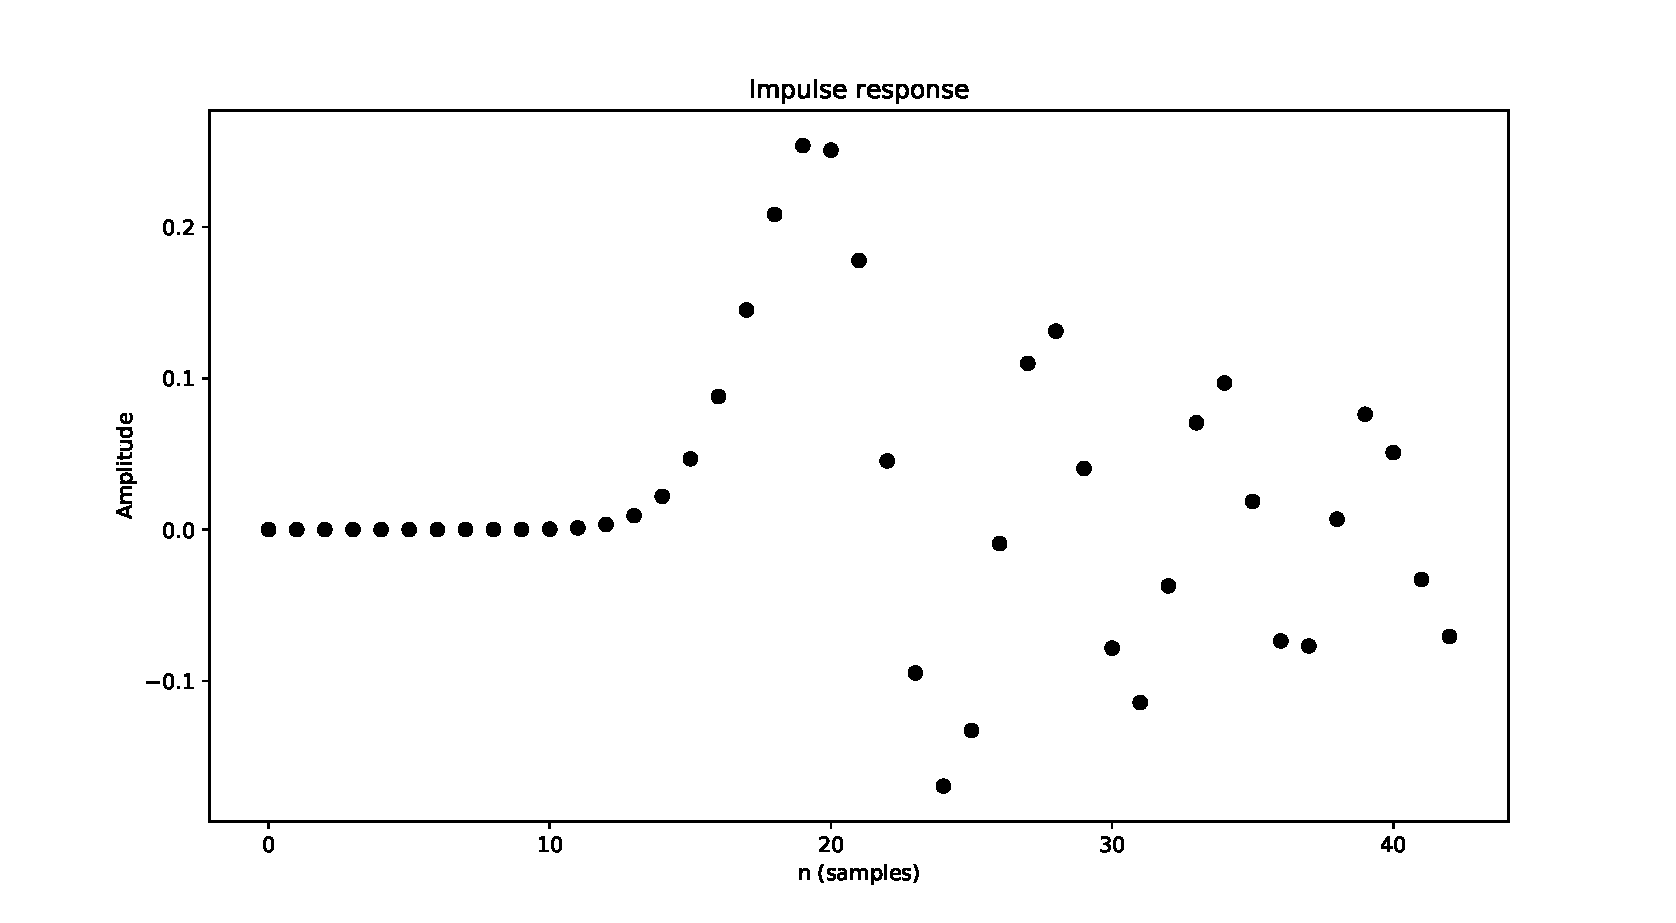
\includegraphics[scale=.4]{Figure_3.pdf}
\caption{Plotted above is the impulse response, h[n], for a Butterworth filter of low-pass type.  The y-axis indicated the coefficient value.}
\end{figure} 
\begin{figure}[!ht]
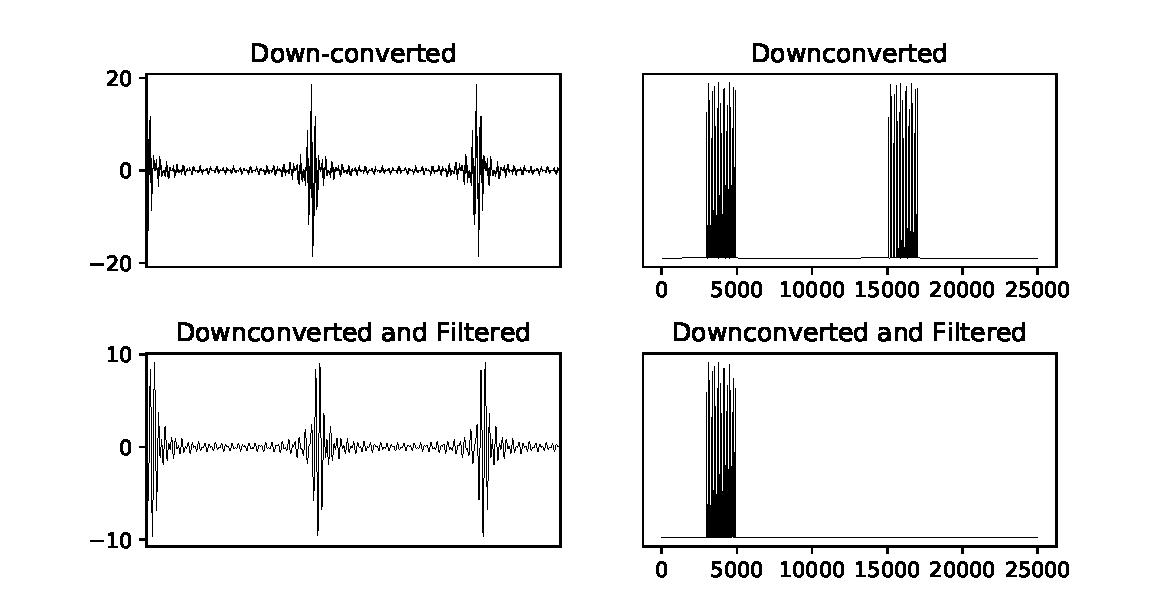
\includegraphics[scale=.6]{Figure_5.pdf}
\caption{(top) Downconverted signal and its Fourier Transform.  (bottom) Downconverted and filtered signal and its Fourier Transform.}
\end{figure} 



\section{Summary}
In this section, we have gone through the steps a signal takes after being measured by a front end system and converted to a digital signal.  This process involves sampling as a given rate, downconverting to a lower/higher frequency band, filtering to remove the high frequency component, then decimating the low frequency result.  As one can imagine, this process can be very hardware expensive.  Are there ways to make this process more efficient? It happens to be the topic of this paper.


\chapter{Polyphase Implementation}

Up to this point, we have discussed the individual components that make up digital signal processing.  What, then, is a polyphase filter bank?  A polyphase filter bank (PFB) is a method of deconstructing the input signal and filter in order to more efficiently carry out the convolution-decimation process which was outlined above.  In a direct implementation, as will be shown below, several of the multipications and additions are unnecessary, and will be discarded during the decimation process.  The PFB allows one to avoid these extra calculations, thus limiting the amount of hardware needed, which is especially important when utilizing finite-space FPGA boards.
\section{Theory}
This section will rely heavily on a paper by (Schafer and Rabiner, 1973), wherein they describe a method for perfect reconstruction across a signal band by a series of bandpass filterings.  They begin by defining the series of bandpass filters as 
\begin{equation}
h_k(n) = h(n)cos(w_kn)
\end{equation}
where $\omega_k=\triangle\omega * k$, $\triangle\omega$ is the distance between center frequencies of adjacent bands, and k is an integer value.  The filter for the entire band is then
\begin{equation}
\widetilde{h}(n) = \sum_k^M h_k
\end{equation}

which, when substituted in, yields
\begin{align}
\widetilde{h}(n) = h(n)\sum_k^M cos(w_kN)
& = h(n)d(n)
\end{align}

Schafer and Rabiner realized that if $\triangle \omega = \frac{2\pi}{NT}$, and $M = \frac{N-1}{2}$, where M is the number of channels, then 
\begin{equation}
d(n) = \frac{sin(\pi n)}{sin(\frac{\pi n}{N})}
\end{equation}

They go on to show that if one were to introduce a delay in d(n), they can remove phase echos which occur during the filtering process.  The relation to the implementation below is reasonable.  We split the filter and signal into subfilters and subsignals, as they have done with the channels.  We then time delay the filters relative to one another, as they show here, and as (Harris, 2003) shows.  In (Harris, 2003), this time delay is given as an unit delay, however.  Another unresolved issue is that, for Schafer and Rabiner, they choose the lowpass filter to be zero at integer multiples of the integer N, which is a function of the number of channels.  It became unclear as to how this should be implemented in the breakdown of the filter into subfilters.
\section{2-tap Example}
This section provides a mathematical walkthrough of a simple 2-tap polyphase implementation.  It suffices to exhibit the time delay which the second filter must have in order to recover the same output as the direction convolution-decimation. 
In a direct computation of the convolution of a signal/filter pair, as shown in Figure 3.1, where the signal is $x[n] = \{x_0, x_1, x_2, x_3, x_4, x_5\}$, and the filter is $h[n] = \{h_0, h_1, h_2, h_3\}$, where the lengths are L=6 and M=4, respectively,
\bigskip
\begin{figure}[ht]
\begin{center}
  \begin{tabular}{ l|c|c|c|c|c|c|c|r }
    \hline
    $h_0 x_0$ & $h_0 x_1$ & $h_0 x_2$ & $h_0 x_3$ & $h_0 x_4$ & $h_0 x_5$ & 0 & 0 & 0\\ \hline
    0 & $h_1 x_0$ & $h_1 x_1$ & $h_1 x_2$ & $h_1 x_3$ & $h_1 x_4$ & $h_1 x_5$ & 0 & 0\\ \hline
    0 & 0 &$h_2 x_0$ & $h_2 x_1$ & $h_2 x_2$ & $h_2 x_3$ & $h_2 x_4$ & $h_2 x_5$ & 0\\ \hline
    0 & 0 & 0 &$h_3 x_0$ & $h_3 x_1$ & $h_3 x_2$ & $h_3 x_3$ & $h_3 x_4$ & $h_3 x_5$ \\\Xhline{1pt}
    $y_0$ & $y_1$ & $y_2$ & $y_3$ & $y_4$ & $y_5$ & $y_6$ & $y_7$ & $y_8$\\ \hline
  \end{tabular}
\end{center}
\caption{The above table represents the computations necessary to implement a direction convolution.  Each column in the table is summed to create the $y_i$ coefficients at the bottom.}
\end{figure}


We can easily see that there are 24 multiplications (L*M), and 27 additions (M-1)*(L+M-1).  Now, if we change our sample rate, as shown in Figure 3.2, 

\begin{figure}[!ht]
\begin{center}
  \begin{tabular}{ l|l }
    \hline
    Before Decimation & After Decimation\\ \Xhline{1pt}
	$y_0 = h_0 x_0$ & $y_0 = h_0 x_0$\\ \hline
	$y_1 = h_0 x_1 + h_0 x_1$ & 0\\ \hline 
	$y_2 = h_0 x_2 + h_1 x_1 + h_2 x_0$ & $y_2 = h_0 x_2 + h_1 x_1 + h_2 x_0$\\ \hline 
	$y_3 = h_0 x_3 + h_1 x_2+ h_2 x_2 + h_3 x_1$ & 0 \\ \hline 
	$y_4 = h_0 x_4 + h_1 x_3+ h_2 x_2 + h_3 x_1$ & $y_4 = h_0 x_4 + h_1 x_3+ h_2 x_2 +     	h_3 x_1$\\ \hline
	$y_5 = h_0 x_5 + h_1 x_4 + h_2 x_3 + h_3 x_2$ & 0\\ \hline
	$y_6 = h_1 x_5 + h_2 x_4 + h_3 x_3$ & $y_6 = h_1 x_5 + h_2 x_4 + h_3 x_3$\\ \hline
	$y_7 = h_2 x_5 + h_2 x_4$ & 0\\ \hline
	$y_8 = h_3 x_5$ & $y_8 = h_3 x_5$\\ \hline
  \end{tabular}
\end{center}
\caption{In the above left column are the coefficients produced by the direct convolution, and in the above right the coefficients remaining after a 2-tap decimation (every other sample).}
\end{figure}

we see that large fraction of the multiplications and additions that were carried out have now been thrown away.  Now to show how a polyphase implementation avoids these unnecessary computations.  First, the filter is split into N-tap subfilters, in this case N=2, which gives $h[n]^+ = \{h_0, h_2\}$ and $h[n]^- = \{h_1, h_3\}$.  Then, the filter is convolved with a sub-band of the input signal, $x[n]$, which are $x[n]^+ = \{x_0, x_2, x_4\}$ and $x[n]^- = \{x_1, x_3, x_5\}$, respectively.  These convolutions are shown in Figure 3.3 and 3.4.

\smallskip
\begin{figure}[!ht]
\begin{center}
  \begin{tabular}{ c|c|c|c }
	\hline
	$h_0 x_0$ & $h_0 x_2$ &$h_0 x_4$&0\\ \hline
	0 & $h_2 x_0$ & $h_2 x_2$ &$h_2 x_4$\\ \Xhline{1pt}
	$y^+_0$ & $y^+_1$ & $y^+_2$ & $y^+_3$\\ \hline
  \end{tabular}
\end{center}
\caption{This table represents the convolution of $h[n]^+$ and $x[n]^+$.}
\end{figure}

The number of multiplications has been reduced to twelve.  We have thus reduced the number of multiplications by half, which for a 2-tap decimation seems reasonable.  However, we have also lowered the number of summations, from twenty seven to thirteen.  
\smallskip
\begin{figure}[!ht]
\begin{center}
  \begin{tabular}{ c|c|c|c }
	\hline
	$h_1 x_1$ & $h_1 x_3$ &$h_1 x_5$&0\\ \hline
	0 & $h_3 x_1$ & $h_3 x_3$ &$h_3 x_5$\\ \Xhline{1pt}
	$y^-_0$ & $y^-_1$ & $y^-_2$ & $y^-_3$\\ \hline
  \end{tabular}
\end{center}
\caption{This table represents the convolution of $h[n]^-$ and $x[n]^-$.}
\end{figure}

\smallskip
\begin{figure}[ht]
\begin{center}
  \begin{tabular}{|c|c|l|}
    \hline
    First Filter & Second Filter &Convolution and Decimation\\ \Xhline{1pt}
	$y^+_0=h_0x_0$ & $y^-_{-1} = 0$ & $y^+_0 + y^-_{-1}= h_0 x_0 = \mathbf{y_0}$\\ \hline
	$y^+_1=h_0x_2+h_2x_0$ & $y^-_0=h_1x_1$ & $y^+_1 + y^-_0 = h_0 x_2 + h_1 x_1 + h_2 x_0 = \mathbf{y_2}$\\ \hline 
	$y^+_2=h_0x_4+h_2x_2$ & $y^-_1=h_1x_3+h_3x_1$ & $y^+_2 + y^-_1 = h_0 x_4 + h_1 x_3+h_2 x_2 + h_3 x_1 = \mathbf{y_4}$\\\hline
	$y^+_3=h_2x_4$ & $y^-_2=h_1x_5+h_3x_3$ & $y^+_3 + y^-_2 = h_1 x_5 + h_2 x_4 + h_3 x_3 = \mathbf{y_6}$\\ \hline
	$y^+_4=0$ & $y^-_3=h_3 x_5$ & $y^+_4 + y^-_3 = h_3 x_5 = \mathbf{y_8}$\\ \hline
  \end{tabular}
\end{center}
\caption{The table above shows how the coefficients of the separate convolutions are summed.}
\end{figure}

Now, combining the results of these two separate convolutions as in Figure 3.5, but in the order that the theory suggets, we take the second output to be delayed by a timestep, which effects a spectral folding of sorts, but with the added benefit of the stopband phase offsets destructively cancelling one another (in theory).

\section{Coded Example}

Herein is presented an example Python code which implements a polyphase decomposition of an ideal lowpass filter.  For the filter, an ideal Butterworth lowpass filter from the Python scipy library was utilized, with the passband edge set at 5000 Hz and the stopband edge set at 7000 Hz, with maximum attentuation in the passband of .1 dB and minimum attenuation in the stopband of 37 dB.  This resulted in a 20th order filter.  As a reference for this code, a powerpoint from Binghamton University (Fowler) was consulted.  A key point in this that was not originally taken into account is the sequence with which the signal subbands are multiplied by the filter subbands.  It is not direct, and there are zero pads that are necessary in order to recover the proper coefficients.  Other than the first signal band, the rest of the bands are multiplied with the filter coefficients in reverse order.  This was shown to be the case for the a 4-tap filter in the powerpoint, but I have my doubts whether or not this holds for higher order taps, as is seen in the performace of the 5-tap filter below.

To demonstrate the code, five separate signals were chosen, since there were several edge cases which needed considering.  The first of these signals contained fourty frequency components, separated at 100 Hz, ranging from 0 kHz to 4 kHz. In this case, all frequencies are within the passband, and the polyphase filter seems to behave rather erratically, as shown in Figure 3.6

\begin{figure}[ht!]
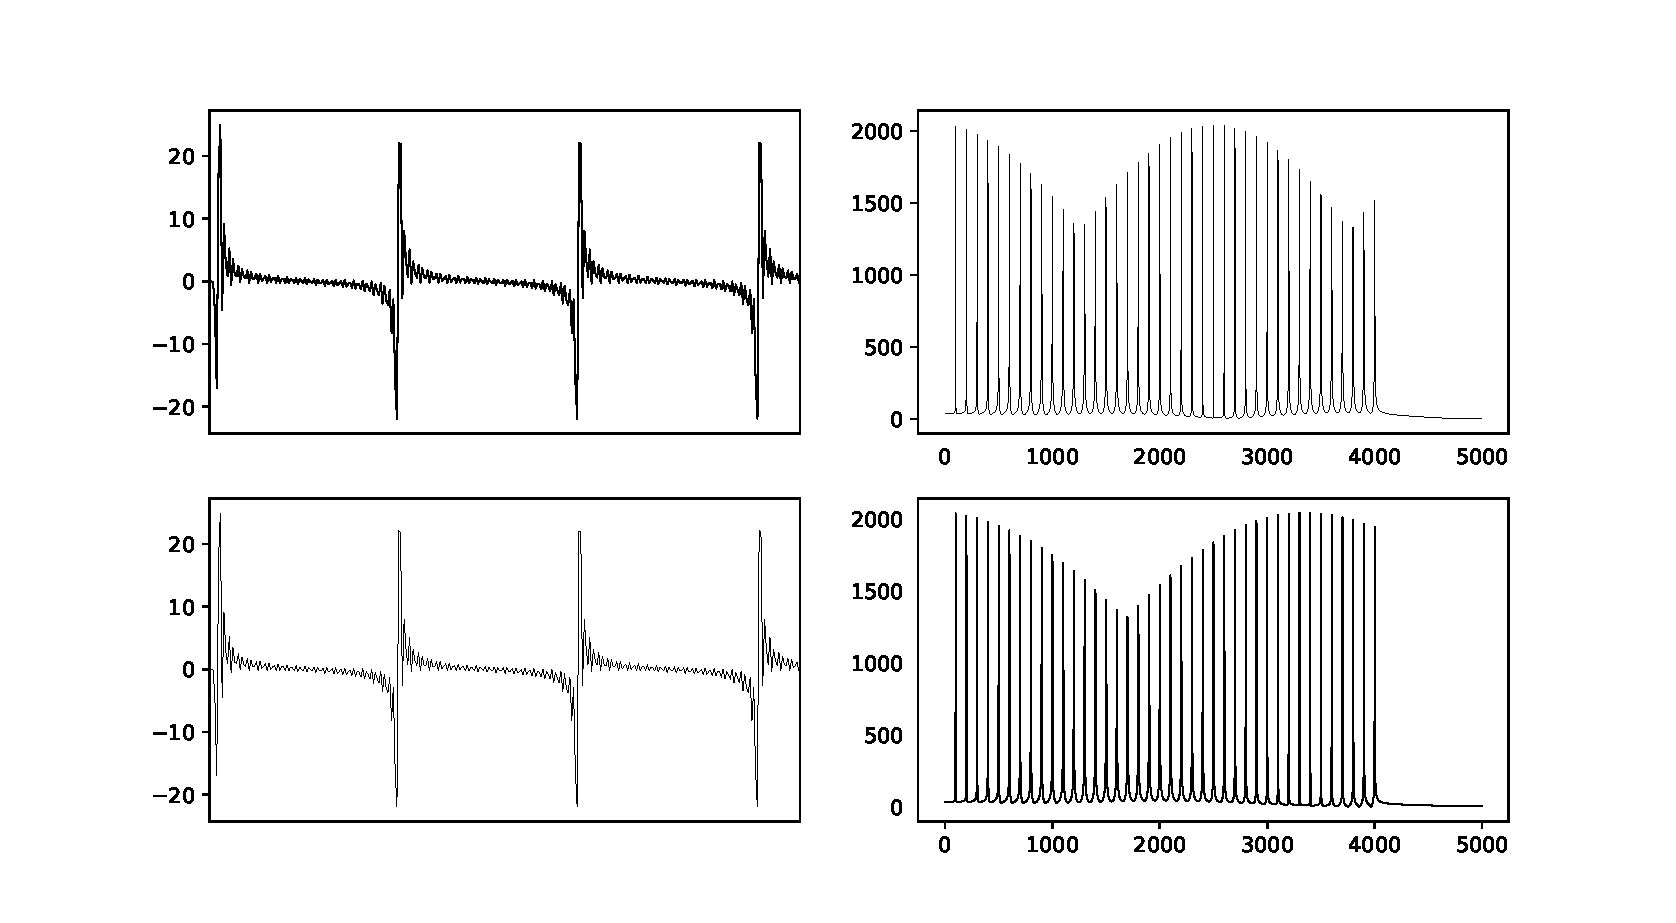
\includegraphics[scale=.6]{Figure_6.pdf}
\caption{(top) is an example of a direct implementation of the Butterworth filter using Scipy lfilter and the Fourier Transform of its output after decimation for the first signal. (bottom) is the polyphase implementation of the same filter on the same signal.}
\end{figure} 

This is the first example which leads to the conclusion that there is still an error in the implementation.  As we see, the response is not flat, as is anticipated in this type of filter bank.  

For the second signal, the number of components was increased to fifty, keeping the same spacing.  The frequencies start at 0 kHz and end at 5 kHz, which completely fills the passband.  The results of this are plotted in Figure 3.7.

\begin{figure}[ht]
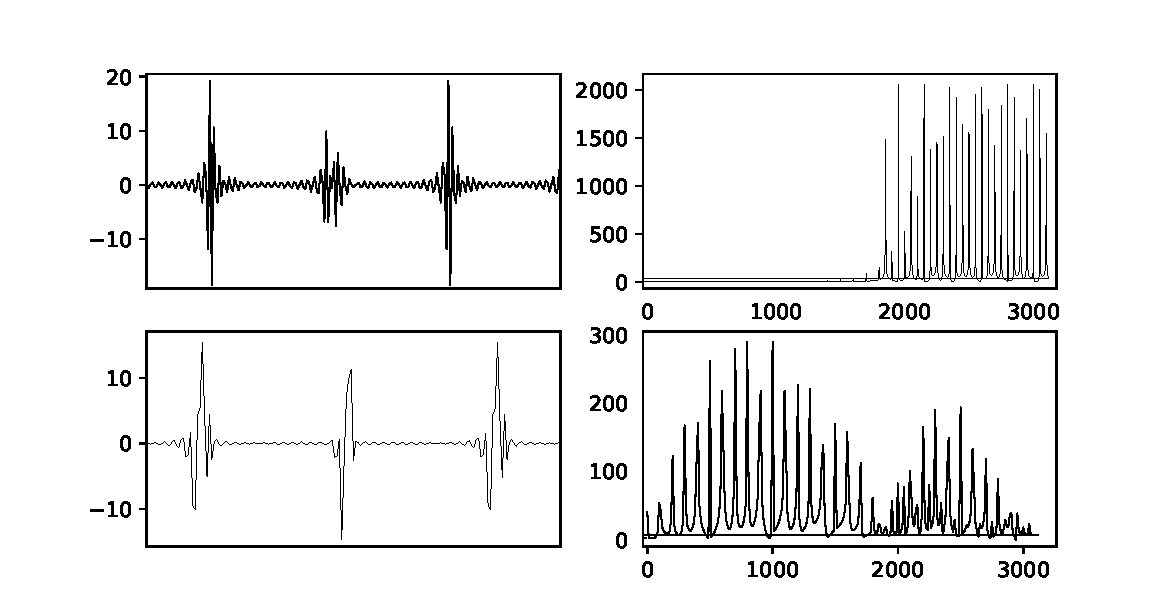
\includegraphics[scale=.55]{Figure_7.pdf}
\caption{Direct (top) vs. Polyphase (bottom) Implementation for second signal}
\end{figure} 

It was not entirely evident how to interpret this result.  Clearly, this is not the flat channel response that was advertised.  We'll save any kibitzing as to possible reasons for the end of this section.

Continuing this trend in the third signal, the component number was increased to sixty.  Now, there is a equally spaced number of components in the passband, and ten components in the transition band. The results of this are shown in Figure 3.8.

\begin{figure}[!ht]
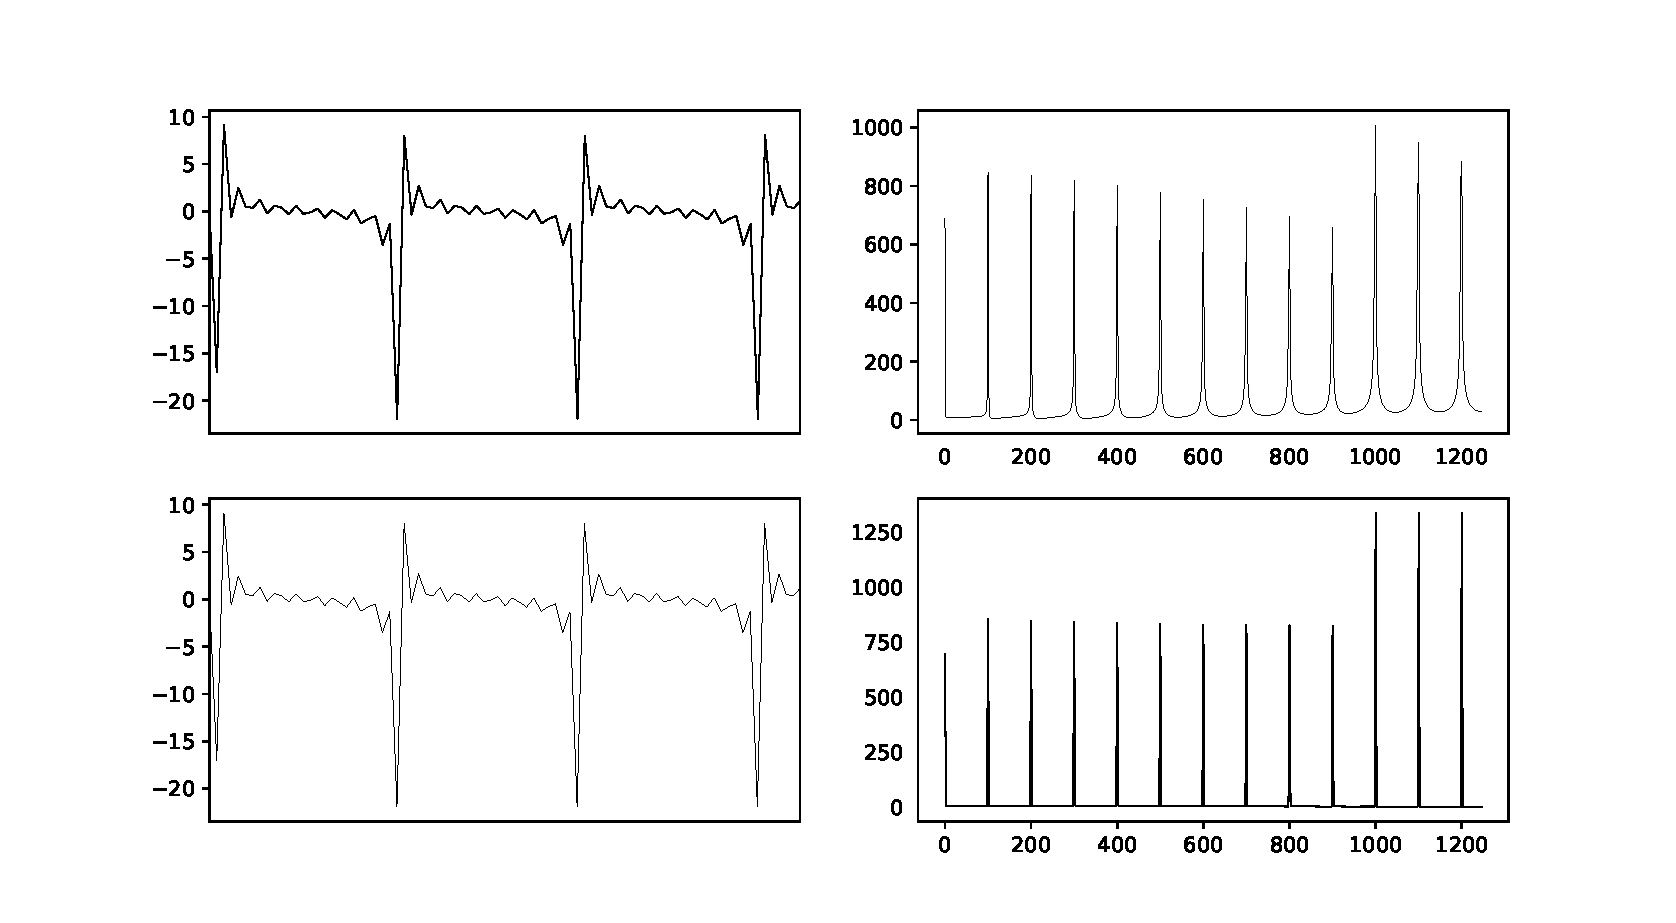
\includegraphics[scale=.55]{Figure_8.pdf}
\caption{Direct (top) vs. Polyphase (bottom) Implementation for third signal}
\end{figure} 

This plot is still puzzling.  It appears that power from frequencies in the transition band are being aliased into the passband, somehow.

\begin{figure}[!ht]
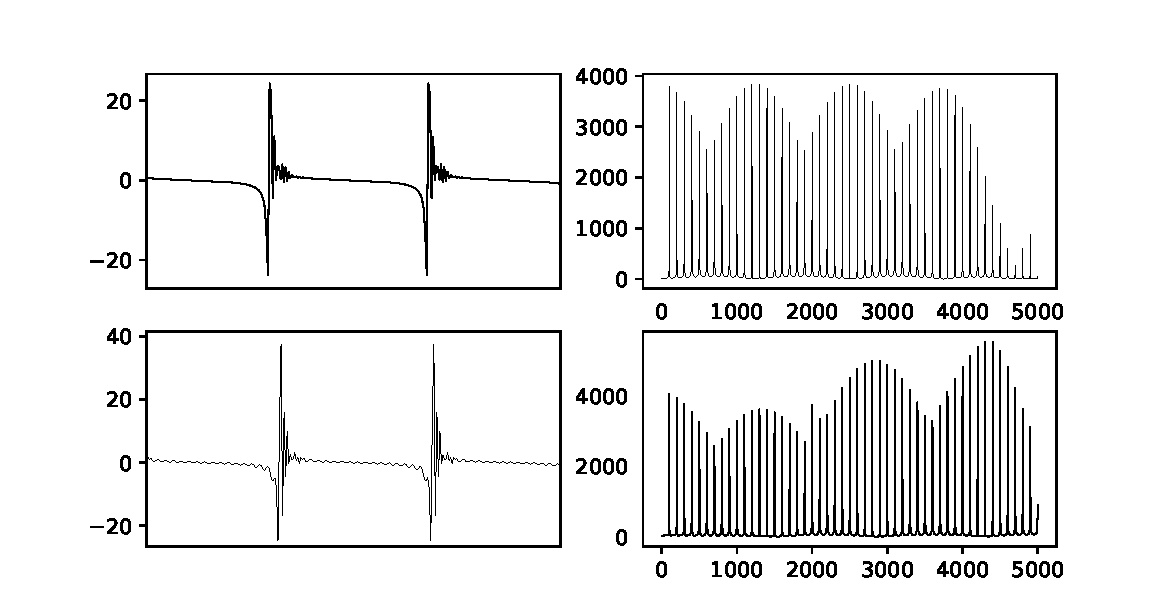
\includegraphics[scale=.55]{Figure_9.pdf}
\caption{Direct (top) vs. Polyphase (bottom) Implementation for fourth signal}
\end{figure} 

For the fourth signal, we again increase the number of components, this time to eighty.  This completely covers the passband, transition band, and gives ten components in the stopband. The results are plotted in Figure 3.9.  This result was almost reassuring, since it does seem to behave better at the channel edge than the direct implementation, but certainly doesn't approach the flat responses which have been seen elsewhere (Schafer, 1973), (Harris, 2003).  

In the fifth rendition, we filled the stopband from 7 kHz to 12 kHz with components 100 Hz apart and conducted the filtering.  This result is exemplified in Figure 3.10.

\begin{figure}[!ht]
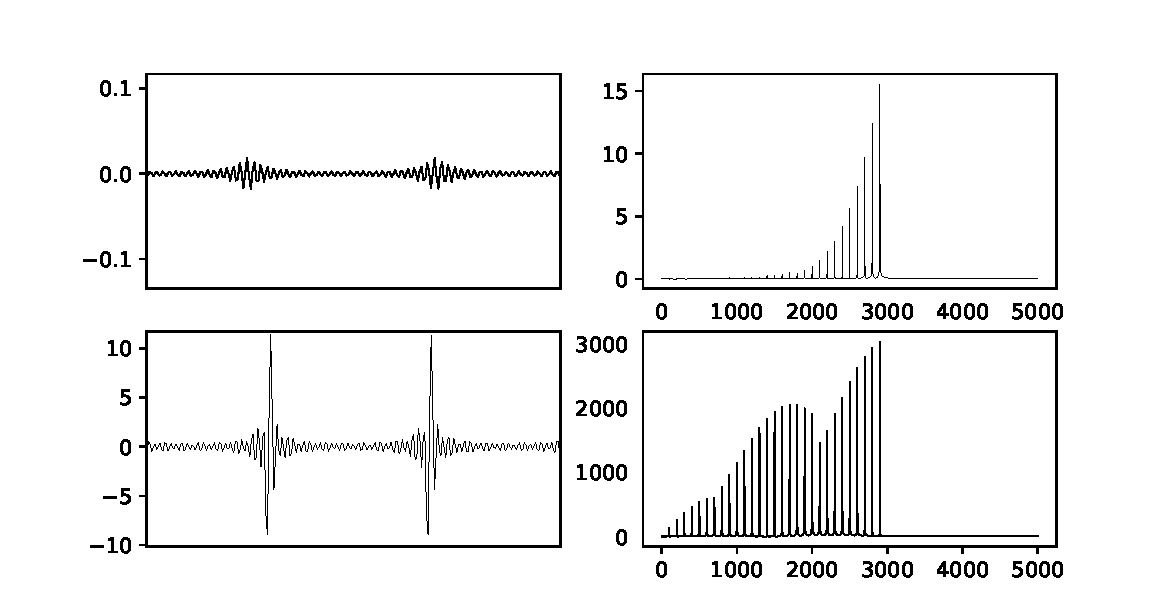
\includegraphics[scale=.55]{Figure_10.pdf}
\caption{Direct (top) vs. Polyphase (bottom) Implementation for fifth signal}
\end{figure} 
 
This was the last signal chosen, since it definitively shows that this implementation is not working.  The direct implementation attenuates the signal very low, as it should, but again it appears that the polyphase implementation is, frustratingly, aliasing the stopband frequencies into the passband.

Before a discussion of what may have gone wrong, we give the code which was utilized above.

\#--------------------------------------------------------------------------------------

\# Implementation of a polyphase downsampler

M = 5

N = 10*4096

signal = FDMSig[500:N+500,0] 

sbl = int(signal.shape[0]/M)

sigBands = np.zeros([sbl + 1,M])

sigBands[:sbl,0] = signal[::M]

for i in range(1,M):

    sigBands[1:,M-i] = signal[i::M]


fbl = int(resp.shape[0]/M)

filtBands = np.zeros([fbl, M])

for i in range(0,M):

    filtBands[:,i] = resp[i::M]

    
subConv = np.zeros([sbl + 1, M])

for i in range(0, M):

    subConv[:, i] = sig.lfilter(filtBands[:,M-i-1], 1, sigBands[:,i])


subConv = subConv.transpose()

polyPhaseOut = subConv.sum(axis=0)

'''
Implementation of filtering, then downsampling
'''

filtSig = sig.lfilter(b, a, FDMSig[:,0])

decFiltSig = filtSig[::M]

\#-------------------------------------------------------------------------------------

Here I have omitted the code used to create the signal.

\section{Discussion/Future Plans}

So, clearly something has gone wrong in this implementation.  The possibilities are quite numerous, and have caused a great deal of owrry in the writing of this report.  Firstly, the Scipy lfilter function was used to implement the filtering.  This is slightly different from a direct convolution.  However, switching the code to a direct convolution setup does little to help the issue of the filter not attenuating signal outside the passband.  The second, and arguably most likely, is I have misunderstood the purpose/implementation of the process.  I attempted to gather several sources and use their approach as best as possible.  I have no doubts as to the deconstruction of the input signal and the filter coefficients, nor that the filter coefficients perform as expected.  I expect that the order reversal demonstrated in the powerpoint is simply not as simple as shown there, which would account for power not within the passband leaking in.  The third possibility is numerical error in the filter deconstruction, but upon inspection these subfilters appear reasonable, and are plotted in Figure 3.11.

\begin{figure}[!ht]
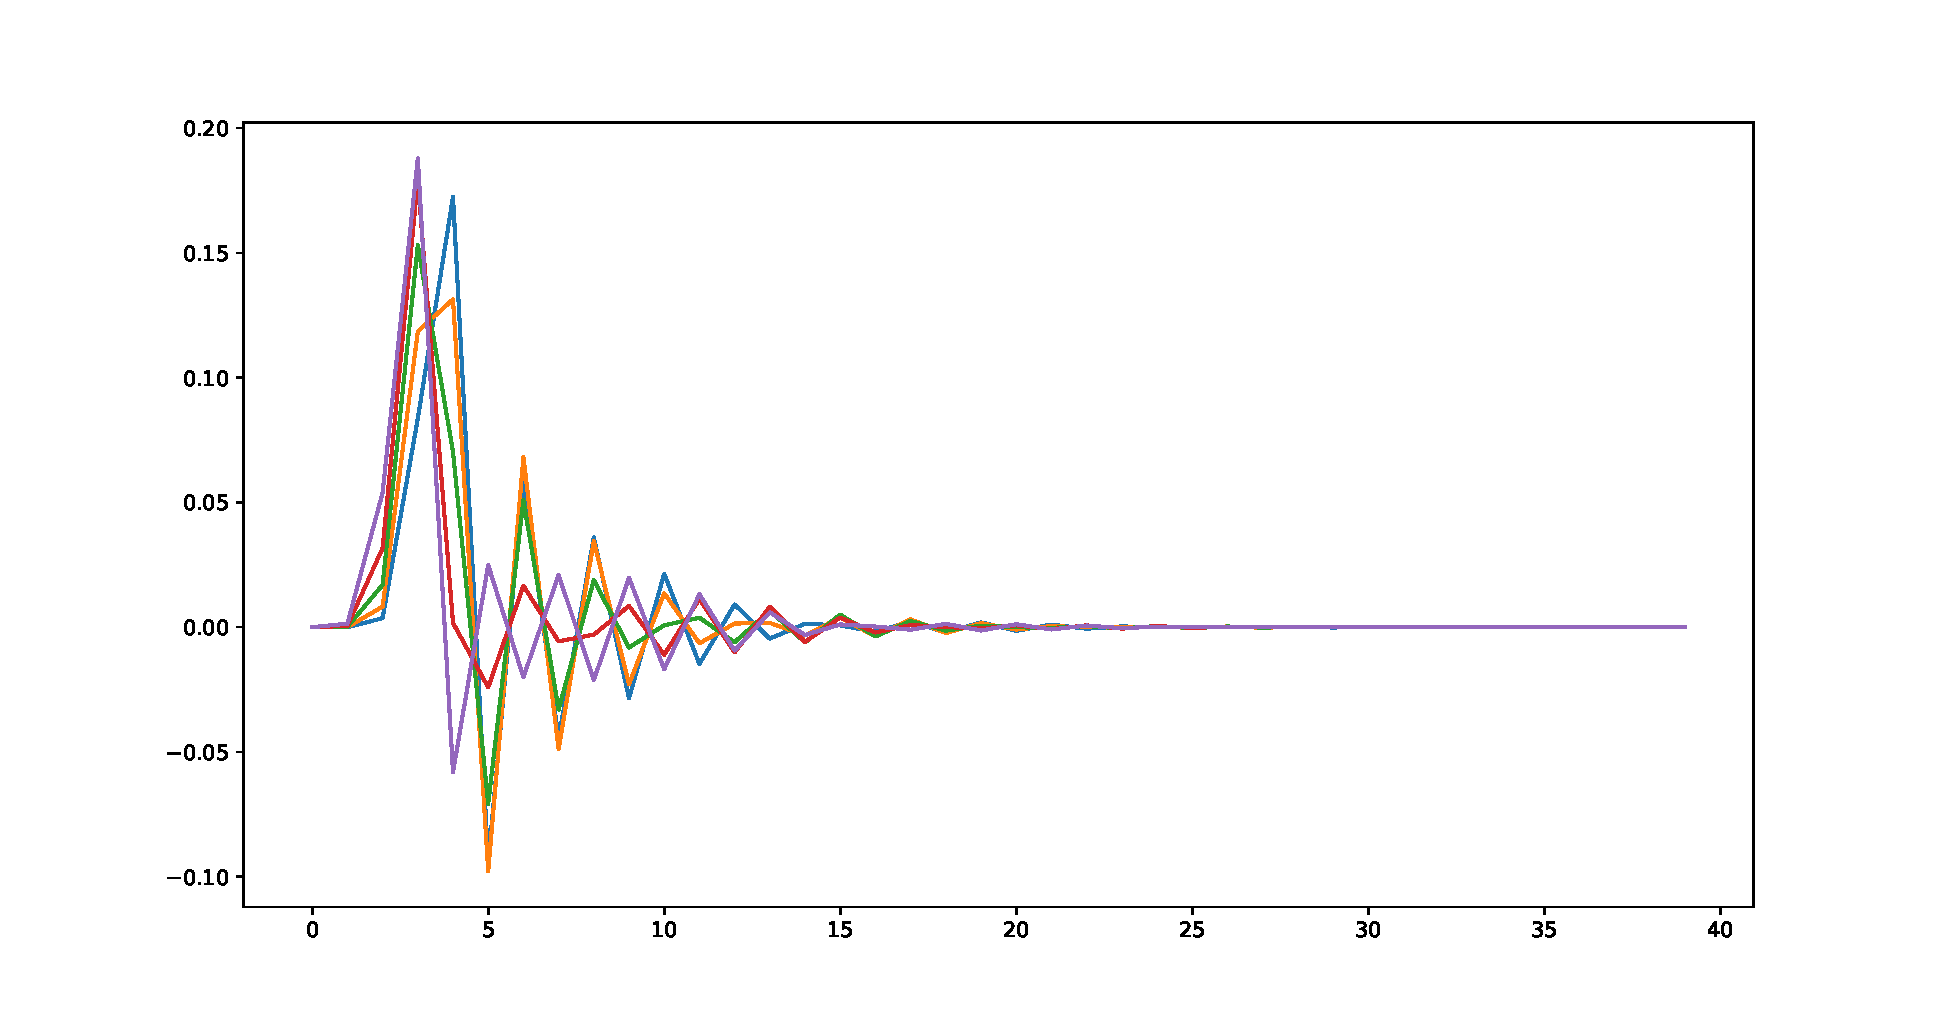
\includegraphics[scale=.4]{Figure_11.pdf}
\caption{Filter subbands for the 5-tap implementation.}
\end{figure} 

The plot thickens, as this implementation doesn't even work with a 4-tap, which is what was suppose to be the safe case.  Another possibility is that this only works for filters with extremely small transition bands, of which the Butterworth is notoriously bad.  But still, it should behave moderately well regardless.  Again, my gut instinct is that the cross convolution is not as straightforward as was suggested in the reference material, barring any bugs in my code that I happen to overlook (if I could be so lucky!).  Future plans are to take a long nap, and then explore a larger example implementation using Matlab's symbolic library, to double check the time reordering in larger N-tap cases, to verify that the time ordering implemented here is correct, though honestly it seemed to check out with a cursory logical nod.

\chapter{Conclusion}

It is hoped that, although this implementation wasn't effective, it has been a solid second step in distilling the information on polyphase filter banks from the extensive literature on the subject, as well as an insight into how such an implementation should be structured.

Well, Dr. Gary, I gave it my best shot, and seemed to have come up short, though I believe I'll be able to correct this and have a functional implementation once I understand the coefficient re-ordering.  I don't plan on giving up, though unfortunately I didn't have enough time to hunt down the error and get this report to you.  

\newpage

\textbf{Bibliography}

Fowler \url{http://www.ws.binghamton.edu/fowler/fowler%20personal%20page/EE521_files/IV-05%20Polyphase%20FIlters%20Revised.pdf}

F. J. Harris, C. Dick and M. Rice, "Digital receivers and transmitters using polyphase filter banks for wireless communications," in IEEE Transactions on Microwave Theory and Techniques, vol. 51, no. 4, pp. 1395-1412, April 2003.

H. J. Landau, "Sampling, data transmission, and the Nyquist rate," in Proceedings of the IEEE, vol. 55, no. 10, pp. 1701-1706, Oct. 1967.
doi: 10.1109/PROC.1967.5962

J.H., Jr, Hammond,  Purington, E.S.. (1957). A History of Some Foundations of Modern Radio-Electronic Technology. Proceedings of the IRE. 45. 1191 - 1208. 10.1109/JRPROC.1957.278525. 

L. C. Godara, "Introduction to "The heterodyne receiving system, and notes on the recent Arlington-Salem tests"," in Proceedings of the IEEE, vol. 87, no. 11, pp. 1975-1978, Nov. 1999.
doi: 10.1109/JPROC.1999.796359

Pal, Srikanta  J. Lancaster, Michael D. Norrod, Roger. (2012). HTS Bandstop Filter for Radio Astronomy. Microwave and Wireless Components Letters, IEEE. 22. 236-238. 10.1109/LMWC.2012.2193122. 

R. W. Schafer and L. R. Rabiner, "A digital signal processing approach to interpolation," in Proceedings of the IEEE, vol. 61, no. 6, pp. 692-702, June 1973.
doi: 10.1109/PROC.1973.9150


\end{document}
